\documentclass{article}
%基于北京航空航天大学仪器科学与光电工程学院实验报告及课程报告排版得来,类似于毕业论文排版格式
%后续将更新毕业论文排版格式
\usepackage{graphicx,float}%使用图的宏包,使用图的浮动体宏包,引入参数H使图像紧跟当前文字
\usepackage{caption} %使用图表标题的宏包
\usepackage[colorlinks=true,pdfstartview=FitH,%
linkcolor=black,anchorcolor=violet,citecolor=magenta]{hyperref}%加载hyperref宏包,使用超链接
\usepackage{setspace}%用于设置行间距列间距等命令的宏包
\usepackage{array}%设置列表高度宽度的宏包
\usepackage{zhnumber}%使用中文数字编号的宏包
\usepackage{titlesec,titletoc}%使用标题自定义形式的宏包和使用目录自定义形式的宏包
\usepackage{siunitx}%物理学单位宏包
\usepackage{tabularx}%让表格宽度等于页面宽度
\usepackage{makecell}%单个表格单元调整的宏包
\usepackage{subfigure} %%使用子图的宏包
\usepackage[backend=biber,bibstyle=gb7714-1987,%nature,%%加载biblatex宏包,使用参考文献
citestyle=gb7714-1987%,backref=true%%其中后端backend使用biber
,url=false
]{biblatex}%标注(引用)样式citestyle,著录样式bibstyle都采用gb7714-2015样式
% \usepackage{pgfplots}%类似tikz的一个画图库,主要画统计图
\usepackage{../customStyle}

\graphicspath{{./fig}}

\fancyhf{} 
% 页眉页脚设置
\lhead{陈博非}
\chead{实验室服务器使用说明}
\rhead{\today}
\cfoot{\thepage}
\rfoot{}
\lfoot{}

% 表格行间距调整为1.5
\renewcommand{\arraystretch}{1.5}

\begin{document}
% 加入页眉页脚
\thispagestyle{fancy}
\section{服务器基本情况}
实验室现有两台服务器,其基本信息如表\ref{tab:server}所示:
\begin{table}[H]
  \centering
  \caption{服务器基本信息}
    \begin{tabular}{ccccccc}
      \toprule
       序号&IP地址& 端口 & 系统版本 & CPU & 内存& 显存 \\
      \hline
      \#1& 10.131.150.189& 20022& Ubuntu18.04&  Intel(R) Xeon(R) Silver 4215R CPU& 192GB& 3090 $\times$8 \\
      \#2&10.131.150.189 &20023&Ubuntu20.04& Intel Core(TM) i9-9900X CPU & 64GB & 2080Ti $\times$4\\
       \bottomrule
  \end{tabular}
  \label{tab:server}
\end{table}
两台服务器当前都位于学院路简易房内,由学校开放校园网网关接入校园网中,可直接使用SSH连接,远程使用。同理,实验室内网也接入校园网,亦可以通过内网直接连接服务器。
\section{你的账号}
基本信息如表\ref{tab:user}所示。
\begin{table}[H]
  \centering
  \caption{账号信息}
  \resizebox{\linewidth}{!}{
  \begin{tabular}{cccc}
      \toprule
       用户名& 密码 & 权限 & 服务器 \\
      \hline
       \code{a804\_qkf} & \code{123456} & 普通用户& \#2\\
       \bottomrule
  \end{tabular}}
  \label{tab:user}
\end{table}
\section{快速使用说明}
\subsection{远程连接}
在Windows本地端连接至服务器,可参考以下步骤:
\begin{enumerate}
  \item 打开命令行cmd,输入\code{ssh -p 20023 a804\_qkf@10.131.150.189}。
  \item 输入密码,即可连接至服务器
\end{enumerate}
如使用\code{pycharm}、\code{vscode}等IDE,可查询相关教程,只要此处能登录,教程内的方法即可使用,此处不再多言,登录后的界面如图\ref{fig:成功登录界面}所示:
\begin{figure}[H]
  \centering
  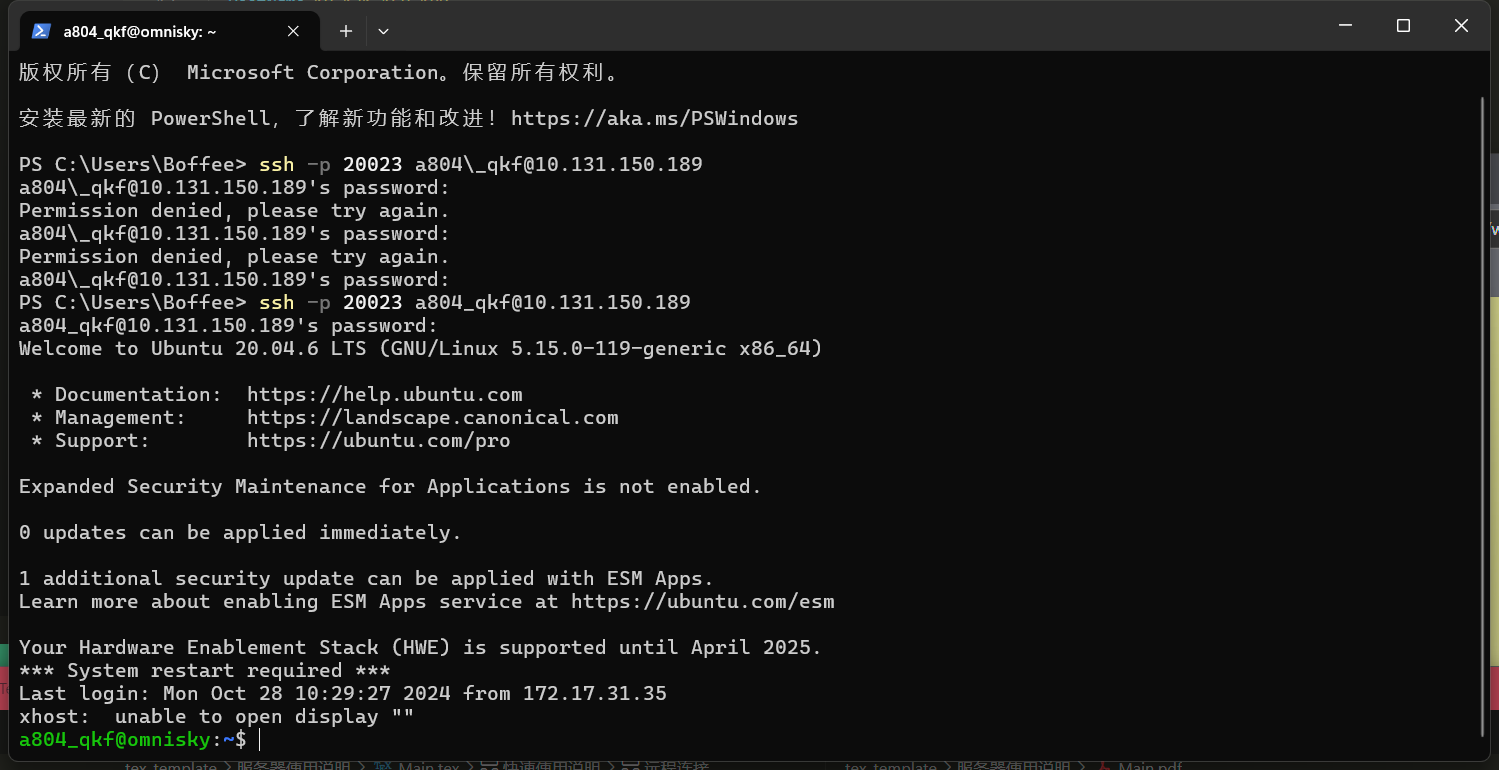
\includegraphics[width=0.8\textwidth]{成功登录界面.png}
  \caption{命令行登录成功界面}
  \label{fig:成功登录界面}
\end{figure}
\subsection{Linux系统快速上手}
使用Linux系统是程序员的基本技能,Linux系统的一大特点是只能通过命令行与操作系统交互。建议熟悉掌握以下常用命令:
  % \resizebox{\linewidth}{!}
  % {
  \begin{longtable}{cc}
    \caption{Linux常用命令}
    \label{tab:Linux常用命令}\\
    \toprule
    命令& 作用\\
    \hline
    \code{cd} & 前往指定目录,如\code{cd /home/a804\_qkf}\\
    \code{ls} & 列出当前目录下的文件,更常用的是它的快捷键\code{ll},可列出详细信息\\
    \code{mv} & 移动文件至另一目录、重命名\\
    \code{cp} & 复制文件\\
    \code{rm} & \makecell[c]{删除文件,加入参数\code{-r }可递归地删除文件夹\\ \textbr{注意!删除一定慎重,服务器上没有启用回收站功能,删除后文件将不可找回}}\\
    \code{mkdir} & 创建文件夹\\
    \code{touch} & 创建文件\\
    \code{|} & 管道运算符,搭配\code{grep}、\code{xargs}、\code{sed}等命令食用更佳\\
    \code{cat} & 查看文件内容\\
    \code{vim} & 编辑文件,\code{vimtutor}可查看教程\\
    \code{top} & 查看系统资源使用情况\\
    \code{ps} & 查看进程\\
    \code{kill} & 杀死进程\\
    \code{scp} & \makecell[c]{从服务器下载文件至本地,亦可上传文件至服务器\\ 如\code{scp -P 20023 /home/a804\_qkf/test.txt  a804\_qkf@10.131.150.189}}\\
    \code{ln} & 快速创建软链接\\
    \code{find} & 查找文件\\
    \bottomrule
   
  \end{longtable}
  % }
  
\subsection{注意事项}
\begin{enumerate}
  \item 网上的教程多数没有考虑自定义端口\code{20023},请务必注意。
  \item 可以配置\code{ssh}的\code{config}文件,使得SSH连接可用快捷键、支持直连(不需要重复输入密码),详情请自行google。
  \item 建议登录系统后立即使用命令\code{passwd}修改密码。
\end{enumerate}
\end{document}
